\section{Calculational setup}
\label{sec:setup}

We do it in a way that works.

\begin{figure}[t!]
  \begin{tabular}{ccccc}
    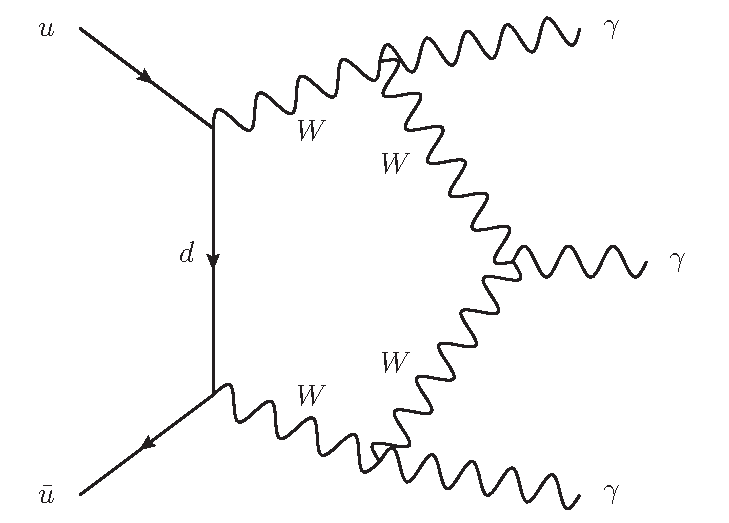
\includegraphics[width=0.3\textwidth]{diagrams/aaa_V_1} & &
    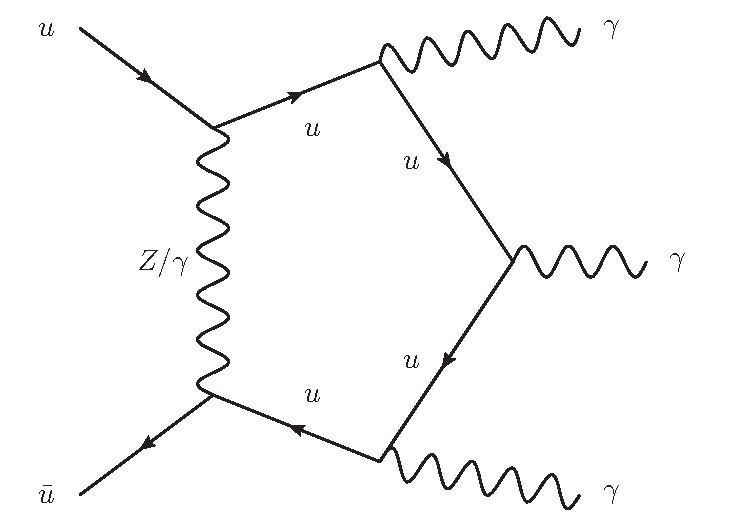
\includegraphics[width=0.3\textwidth]{diagrams/aaa_V_2} & &
    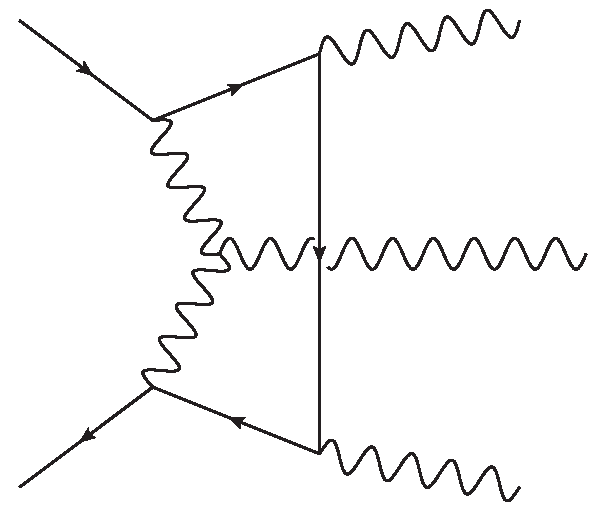
\includegraphics[width=0.3\textwidth]{diagrams/aaa_V_3} \\
  \end{tabular}
  \caption{
    Sample diagrams of electroweak virtual corrections to triple 
    photon production.
  }
\end{figure}

\begin{figure}[t!]
  \begin{tabular}{ccccc}
%     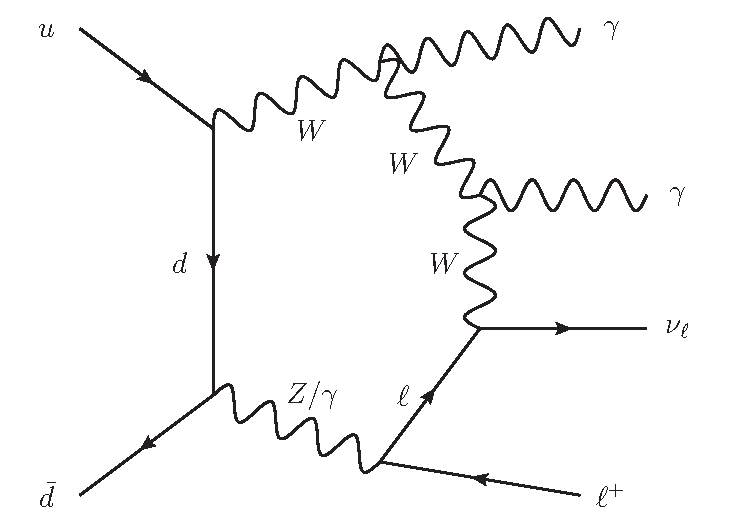
\includegraphics[width=0.3\textwidth]{diagrams/aaW_V_1} & &
%     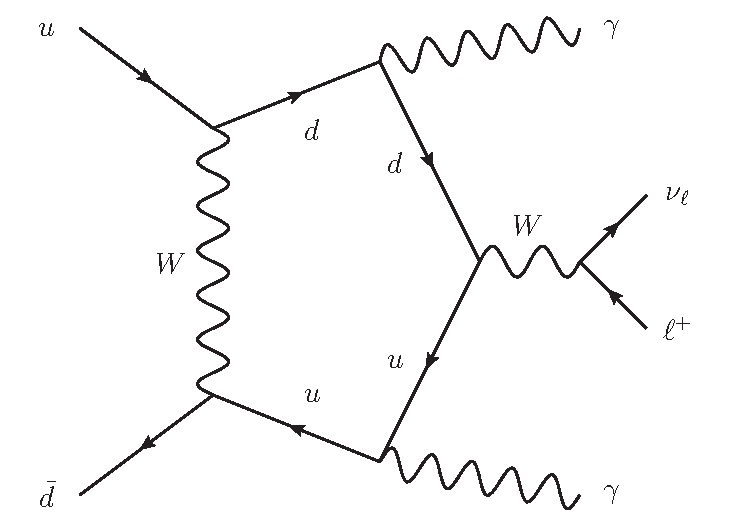
\includegraphics[width=0.3\textwidth]{diagrams/aaW_V_2} & &
%     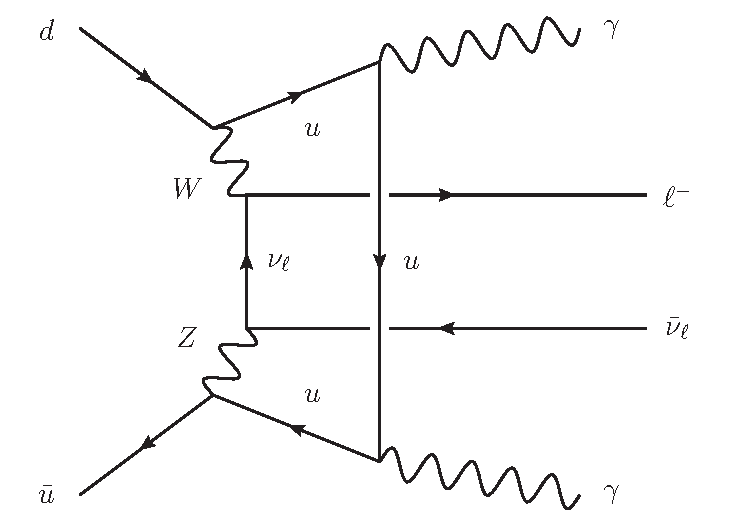
\includegraphics[width=0.3\textwidth]{diagrams/aaW_V_3} \\
  \end{tabular}
  \caption{
    Sample diagrams of electroweak virtual corrections to diphoton 
    production in association with a lepton-neutrino pair.
  }
\end{figure}

\begin{figure}[t!]
  \begin{tabular}{ccccc}
%     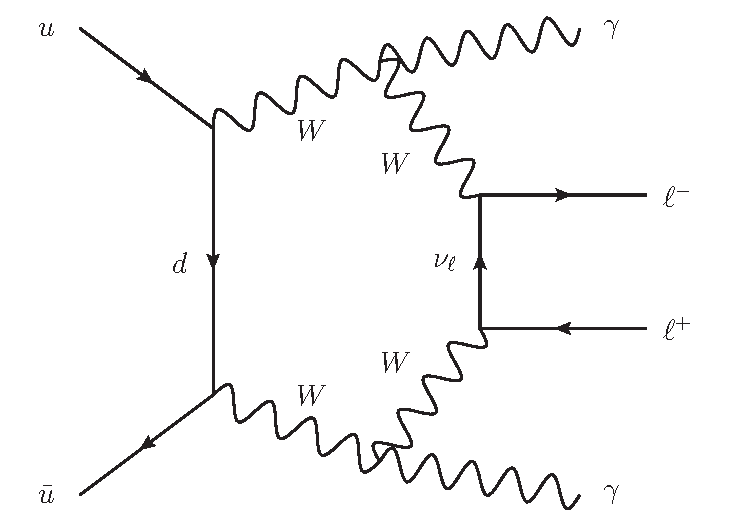
\includegraphics[width=0.3\textwidth]{diagrams/aaZ_V_1} & &
%     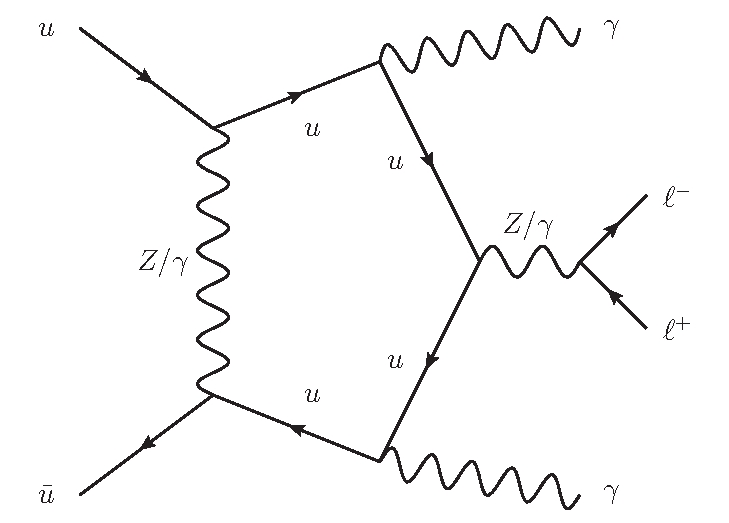
\includegraphics[width=0.3\textwidth]{diagrams/aaZ_V_2} & &
%     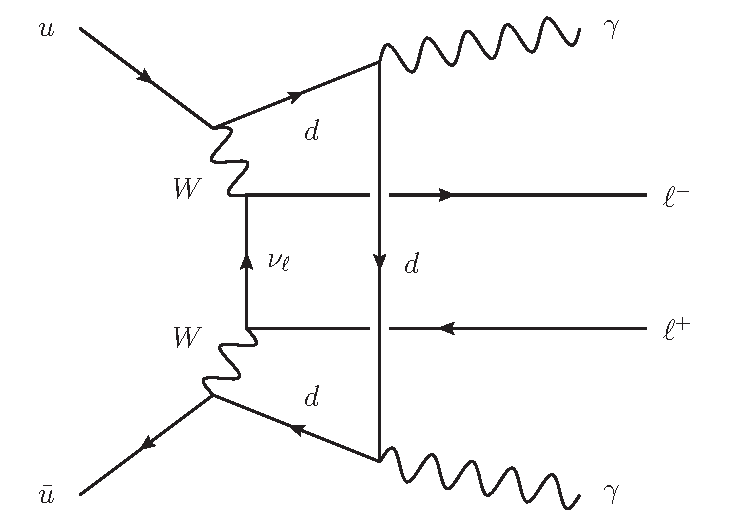
\includegraphics[width=0.3\textwidth]{diagrams/aaZ_V_3} \\
  \end{tabular}
  \caption{
    Sample diagrams of electroweak virtual corrections to diphoton 
    production in association with a lepton-pair.
  }
\end{figure}
